\section{Experimental Protocol}
\subsection*{Optimization Parameters}
An initial pilot was run varying 6 parameters
\begin{table}[h]
  \centering
  \begin{tabular}{ c c }
  Peak Force & Maximum force in Newtons provided\\
  Onset Timing & Start of assistance during the gait cycle\\
  Peak Timing & Point of peak force provided during the gait cycle\\
  Offset Timing & End of assistance during the gait cycle\\
  Curvature 1 & Force provided at midpoint of onset and peak\\
  Curvature 2 & Force provided at midpoint of peak and offset
  \end{tabular}
\end{table}

\subsection*{Hip-only Soft Exosuit}
The textile components of the hip-only soft exosuit consist of a short spandex base layer, a waist belt, and two thigh braces as described in \citep{Lee2018}. Two IMUs (MTi-3 AHRS, Xsens Technologies B.V., Enschede, Netherlands) mounted on the anterior part of the thigh measure the orientation and angular velocity of thigh segments which are used for gait cycle estimation in real-time \citep{Ding2016}. The anchoring points of the Bowden cable are at the bottom left and right of the waist belt as well as at the middle center of the thigh braces from the posterior view. Two load cells (LSB200, Futek Advanced Sensor Technology Inc., CA, USA) are integrated in the aluminum attachment piece of the anchoring point to measure the cable force. When the actuator pulls the inner cable, the soft exosuit generates a hip extension torque by shortening the distance between two anchoring points. 

\subsection*{Actuation System}
The two DOF actuators in the off-board system are used to deliver hip extension assistance to both legs. Each actuator consists of a customized brushless motor (Allied Motion, Colorado, USA), a 9.25:1 spiroid gear set (ITW Heartland, MN, USA) and a 45 mm radius pulley. The pulley groove is designed to be able to wrap the inner Bowden cable 1.5 times around the pulley, allowing 420 mm of cable travel \citep{Lee2018}. A 360 counts/rev incremental encoder (AS5134-ZSST, ams AG, Premstaetten, Austria) is mounted on the customized motor to measure its position and velocity. The Bowden cable sheath of the actuator side connects to the pulley cover and inner cable attaches to the pulley. When the motor rotates, the actuator can either pull in the inner cable to generate a force or push the cable out so it can go slack.

\subsection*{Control System Architecture}
The electronics hardware has a three-layer configuration for the control system architecture: real-time target machine (top layer), microprocessor (middle layer), and servomotor driver (bottom layer). In the top layer, the Speedgoat real-time target machine runs a Simulink model in a host laptop. A PCI interface card (CAN-AC PCI, Softing AG, Haar, Germany) for CAN communication is installed on the target machine to acquire sensor signals and send the command to the servomotor driver through the microprocessor. The microprocessor (Due, Arudino, Ivrea, Italy) in the middle layer acts as a signal hub between target machine and servomotor driver while protecting the system from undesired behavior of the actuator due to anomalous errors from the target machine. In the bottom layer, Gold Twitter (Elmo Motion Control Ltd, Israel) with 55V maximum supply voltage and 60 A peak current is selected as the current servomotor driver. It tracks the current command from the microprocessor to drive the actuator. The CAN communication between layers closes the control loop at 1kHz loop rate \citep{Lee2018}.

Another laptop collects the metabolic data, runs an optimization algorithm, and sends the assistance profile parameters that will be explored in the next condition to the host laptop. Ethernet communication is used between a real-time target machine, a host laptop, and the second laptop. Based on the profile parameters calculated by the algorithm, the host laptop sends the current command to the servomotor drive to deliver assistance to the subject.

\section{Experimental Subjects}
Two male subjects (S1: 27 yrs, 74 kg, 177 cm; S2: 48 yrs, 85 kg, 178 cm) participated in this preliminary study. The subjects walked on the treadmill at 1.25 m/s under four different conditions: Normal walking without Exosuit (N), Exosuit-off (OFF), Fixed Exosuit Assistance (FIX) and Optimal Exosuit Assistance (OPT). During FIX condition, the force profiles assisting hip extension were based on the previous study of \citep{Ding2016}, whereas force profiles in OPT condition were determined through a two-part procedure (8 exploration points, 5 minute break, then 40 minute continuous optimization) which was performed before walking test conditions. Metabolic cost of walking across different conditions was measured using a portable gas analysis system (K4b2, Cosmed, Roma, Italy).

\begin{figure}[t]
\centering
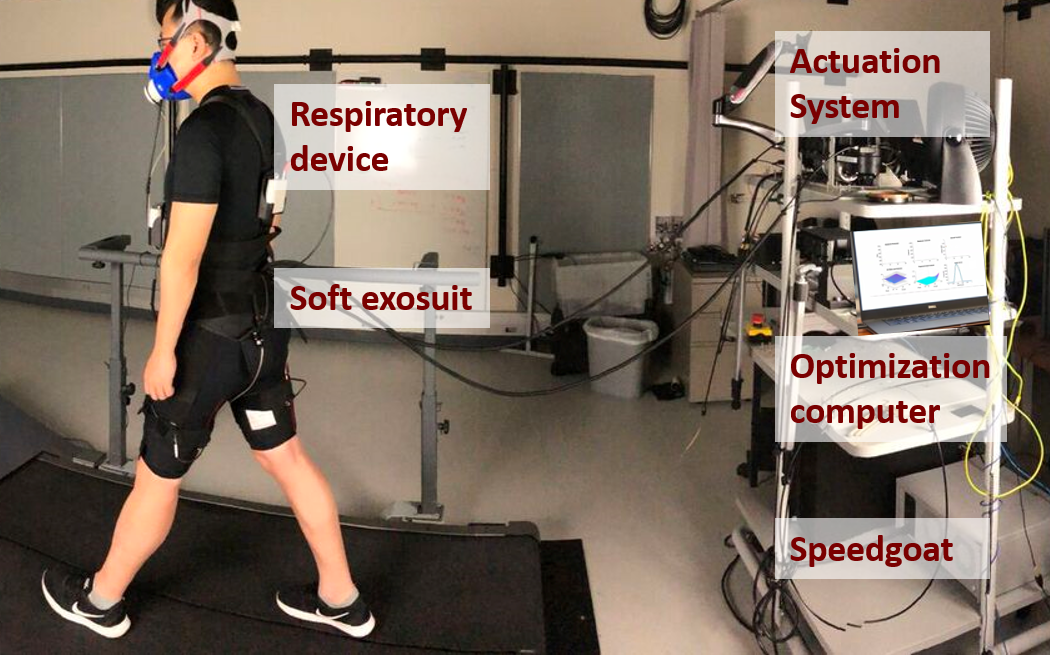
\includegraphics[width=\textwidth]{system_setup.png}
\caption{Experimental setup. Assistance parameters for the soft exosuit were optimized on-line. Respiratory device measured respiratory rate to estimate metabolic cost for a given condition with a covariance. In the optimization computer, the Gittins process determined when to stop sampling and Bayesian optimization was used to select a next parameter set. The parameters were sent to the real-time computer (speedgoat) to generate a force trajectory. Then, the actuator provided a force to a subject through a bowden cables. }
\label{fig:expsetup}
\end{figure}

\section{Results}
Two human trials with the same subjects from a previous study were conducted as a comparison. The Gittins method was used with a relatively risk averse $K=0.35$ to account for the possibility of a very low signal-to-noise ratio, as well as the practical consideration of parameters requiring time to fully propagate to the suit. A summary of the metabolic reduction can be found in Table \ref{fig:expsummary} with figures for the optimized force assistance in Figure \ref{fig:forceprofile}. The soft exosuit followed desired trajectory within 5\% error, relative to the peak force.

\begin{figure}[t]
\centering
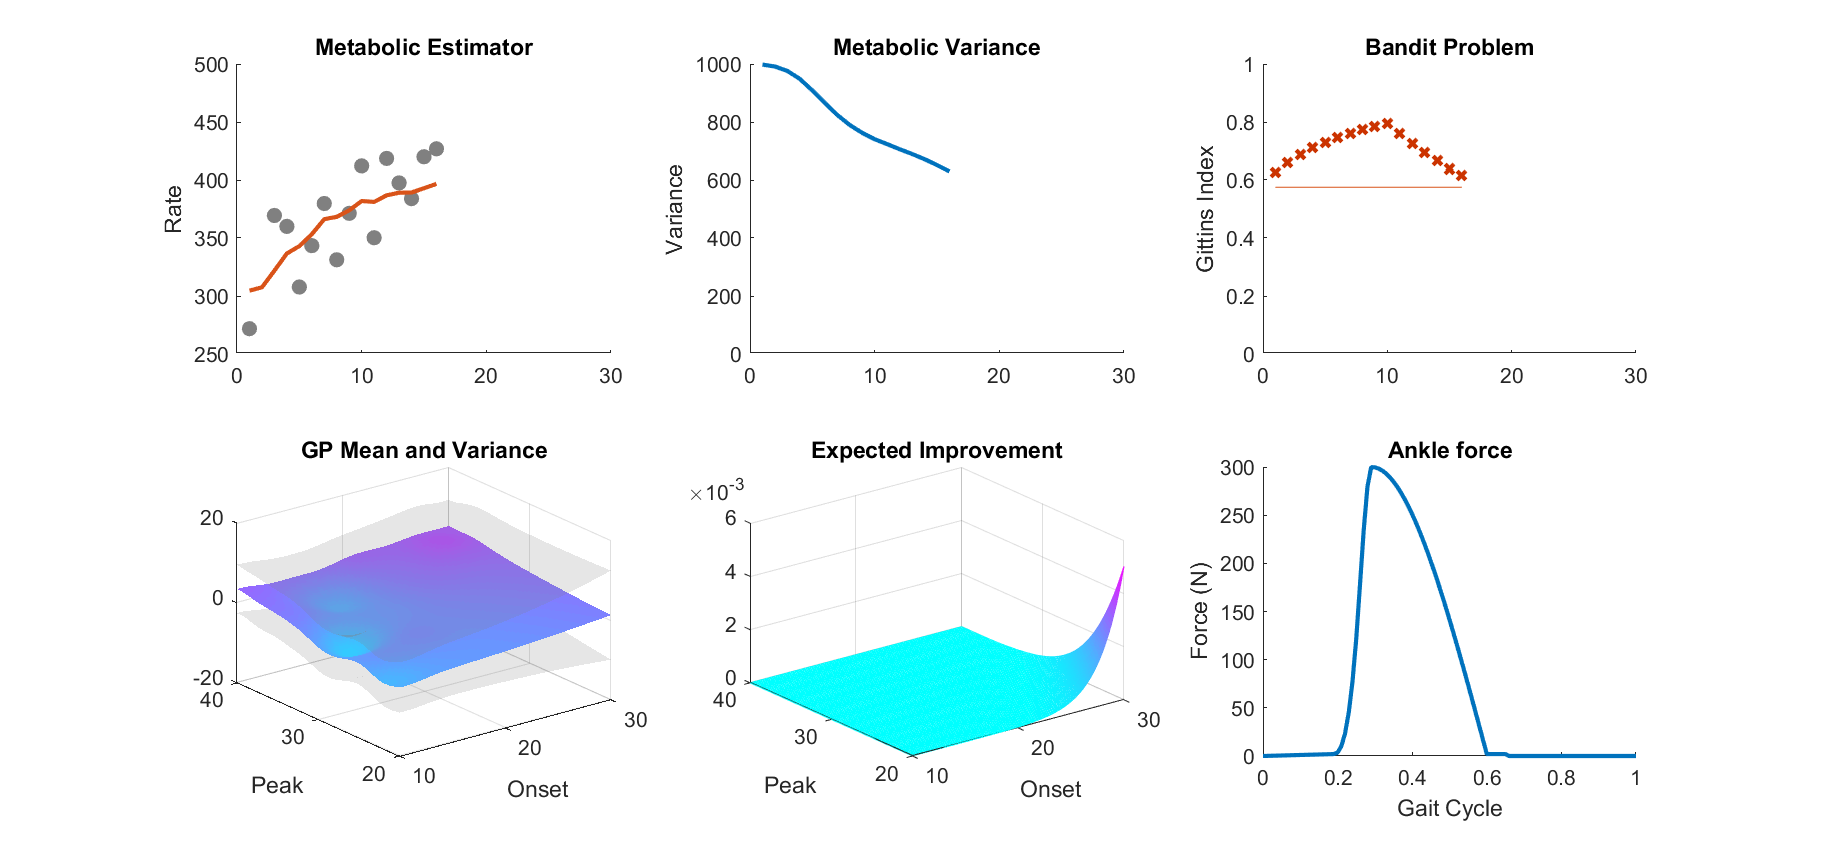
\includegraphics[width=\textwidth]{block}
\caption{Diagram of Bandit Process}
\label{fig:block}
\end{figure}

\begin{table}
\centering
\begin{tabular}{ |c|c|c|c|c|c|c| } 
 \hline
 Subj & OPT & FIX & OPT Peak F & FIX Peak F\\ 
 \hline
 1 & 35\% & 29\% & 223N & 247N\\
 2 & 7\% & -4\% & 174N & 230N \\
 \hline
\end{tabular}%
\caption{Subject Trial Summary}
\label{fig:expsummary}
\end{table}

\begin{figure}[t]
\centering
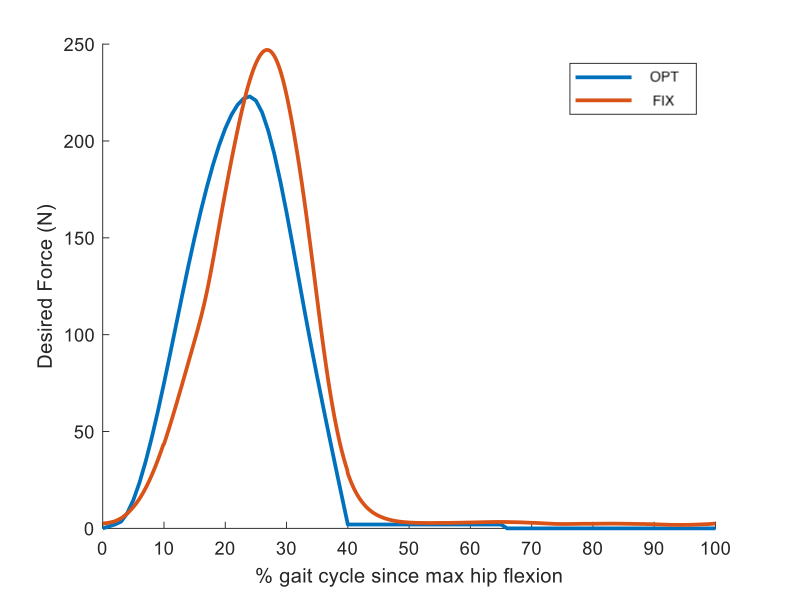
\includegraphics[width=.5\linewidth]{subj1}\hfill
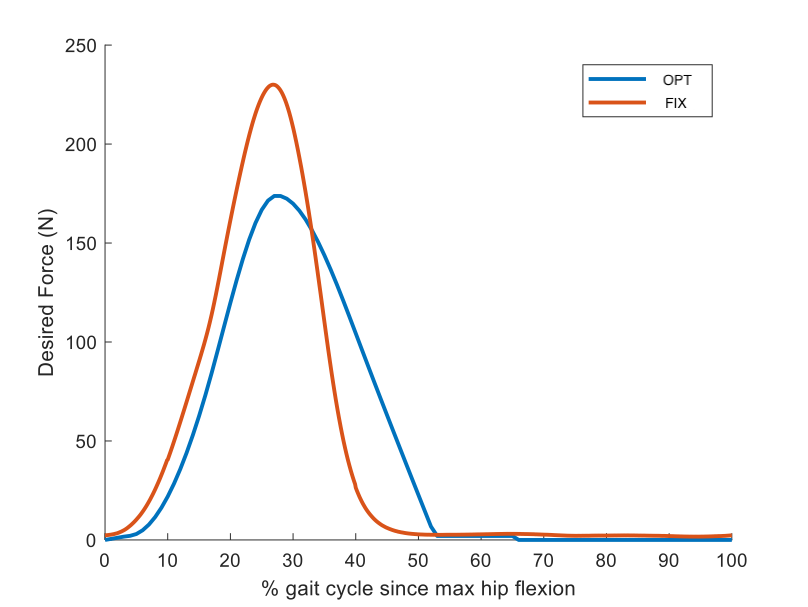
\includegraphics[width=.5\linewidth]{subj2}
\caption{Force profiles of the two subjects}
\label{fig:forceprofile}
\end{figure}

\section{Conclusions}
A new metabolic estimator based off the Unscented Kalman Filter algorithm was designed to enable early stopping for a parameter evaluation. The estimator has shown the ability to track the instantaneous metabolic rate online with varying amounts of data, but is sensitive to the parameterization of it's covariance matrices. Two methods were developed for early stopping: a simple $\sigma$-offset threshold strategy and a bandit process strategy based off the Gittins Index. Depending on the noisiness of the estimator, the bandit process provides a higher fault tolerance for noisy observations. Two trials were then conducted using the Gittins algorithm to optimize over six hip parameters and we found comparable metabolic reduction to a previous study with the same subjects. In the previous study ample time was spent isolating the parameters individually to find the two with high variability (peak and offset timing). While the optimization period for a trial is slightly longer, we were able to find similar results without the need for an extensive pre-trial exploration phase. Interestingly, we also found a lower peak force to provide similar metabolic reduction in each of the two subjects. Having a lower peak force could provide two benefits: lower battery requirements on the suit and more importantly reduced strain on the harness and subsequent discomfort to the user. Future work in this area can focus on tuning the estimator's covariance matrices with exploration phase data and testing more subjects with both models. In particular, an area of interest would be using the algorithm in multi-joint optimization \citep{1298569}.